\documentclass[11pt]{article}

% ─── Page geometry (>=1cm margins per spec) ────────────────────────
\usepackage[margin=1.2cm, top=1.2cm, bottom=1.2cm]{geometry}

% ─── Packages ──────────────────────────────────────────────────────
\usepackage{amsmath, amssymb}
\usepackage{graphicx}
\usepackage{booktabs}
\usepackage{multirow}
\usepackage{enumitem}
\usepackage[font=small, labelfont=bf]{caption}
\usepackage{xcolor}
\usepackage{hyperref}

% ─── Compact spacing ──────────────────────────────────────────────
\usepackage{titlesec}
\titlespacing*{\section}{0pt}{6pt}{3pt}
\titlespacing*{\subsection}{0pt}{4pt}{2pt}
\titleformat{\section}{\normalfont\bfseries\large}{\thesection.}{0.5em}{}
\titleformat{\subsection}{\normalfont\bfseries\normalsize}{\thesubsection}{0.5em}{}
\setlength{\parskip}{2pt}
\setlength{\parindent}{0pt}
\setlength{\abovecaptionskip}{4pt}
\setlength{\belowcaptionskip}{2pt}
\setlist{nosep, leftmargin=1.2em}
\renewcommand{\arraystretch}{1.05}

\begin{document}

% ─── Title ─────────────────────────────────────────────────────────
\begin{center}
    {\Large\bfseries Human vs.\ Machine Text Classification\\[2pt]on Obfuscated Token Sequences}\\[6pt]
    {\normalsize CP219 Machine Learning --- Project~1}\\[2pt]
    % {\normalsize Author Name \quad | \quad IISc, Semester 1, 2026}
\end{center}

\vspace{-4pt}

% ===================================================================
\section{Introduction}
% ===================================================================

We address a binary classification task: given a document represented as a sequence of integer token IDs, determine whether it was written by a \textbf{human} (Class~A) or generated by a \textbf{machine / LLM} (Class~B). The training set contains 10,536 documents (A:~3,699; B:~6,837; imbalance ratio $\approx$1.85:1) over a vocabulary of ${\sim}18{,}438$ token IDs. The test set has 3,000 documents, evaluated on classification accuracy via Kaggle.

A key constraint is that the text is \textit{pre-tokenized}---no raw words, punctuation, or sentence boundaries are accessible. All feature engineering must operate directly on integer sequences. Our best submission achieves \textbf{96.00\% accuracy} on the Kaggle public leaderboard using a 150,027-dimensional feature representation with a LightGBM classifier.

% ===================================================================
\section{Feature Engineering}
% ===================================================================

We construct four complementary feature families, horizontally stacked into a single sparse matrix:

\subsection{TF-IDF N-gram Features (150,000 features)}
Token-ID sequences are converted to whitespace-joined strings and vectorized using \texttt{TfidfVectorizer} with unigrams, bigrams, and trigrams (\texttt{ngram\_range=(1,3)}), 150,000 max features, and sublinear TF ($1 + \log(\text{tf})$). This captures specific token combinations characteristic of AI vs.\ human text while dampening high-frequency tokens.

\subsection{Extended Stylometric Features (18 features)}
Six base features (\texttt{doc\_length}, \texttt{unique\_tokens}, type-token ratio, OOV rate, Shannon entropy, zlib compression ratio) capture document-level distributional statistics. Twelve extended features add bigram entropy, bigram TTR, positional statistics (head/tail mean token IDs), frequency concentration (top-1 and top-5 relative frequency, hapax rate), and vocabulary range (token range, Q25, Q75). These operate without any vocabulary information, providing signal orthogonal to TF-IDF.

\subsection{Generative Markov Features (8 features)}
\label{sec:gen}
This family produced the \textbf{largest single accuracy improvement} (+4.31~pp). Class-conditional bigram and trigram Markov chain transition models are built from the training data, and each document is scored by its log-likelihood under each class model. Transition counts use \textit{Python dictionaries} (not dense $V{\times}V$ matrices, which would require ${\sim}$1.3\,GB for bigrams and ${\sim}$24\,TB for trigrams). Laplace smoothing ($\alpha{=}0.1$) is applied: $P(t_2|t_1) = \frac{C(t_1,t_2)+\alpha}{C(t_1)+\alpha V}$. A \textbf{Leave-One-Out (LOO)} correction subtracts each training document's own contribution before scoring, preventing self-memorization.

The eight features are: \texttt{ll\_human\_bi}, \texttt{ll\_ai\_bi}, \texttt{ll\_diff\_bi} (human$-$machine; the most discriminative signal), and their trigram counterparts, plus a Zipf slope and mean burstiness.

\subsection{Heaps' Law Feature (1 feature)}
The vocabulary-growth exponent $\beta$ (from $V \propto N^{\beta}$) is estimated by log-log regression over ${\sim}$20 sampled points. Humans introduce vocabulary irregularly; LLMs exhibit smoother growth curves.

% ===================================================================
\section{Models}
% ===================================================================

\textbf{LightGBM} (primary): 500 trees, $\text{lr}{=}0.05$, 63 leaves, \texttt{scale\_pos\_weight}{=}1.848, L1/L2 regularization, 80\% row/column subsampling. Systematic \textbf{hyperparameter tuning} via Optuna was attempted but terminated due to excessive runtime on the 150k-dimensional sparse matrix; thus, robust default parameters were maintained.
\textbf{Logistic Regression}: SAGA solver, $C{=}1.0$, balanced weights.
\textbf{LinearSVC}: $C{=}0.1$, isotonic calibration (3-fold).
\textbf{XGBoost}: 500 trees, $\text{lr}{=}0.05$, \texttt{max\_depth}{=}6$.
\textbf{Stacking Ensemble}: OOF probabilities from base models $\to$ LR meta-learner. The ensemble employed \textbf{classification threshold optimization}, tuning the decision boundary from the default 0.5 to an optimal 0.45 to maximize accuracy.

% ===================================================================
\section{Experimental Setup and Results}
% ===================================================================

All experiments use 5-fold Stratified K-Fold CV (\texttt{seed=42}). Feature extractors are fit per-fold to prevent leakage.

\subsection{Baseline Progression}

\begin{table}[h!]
\centering
\caption{Cross-validation results for baseline models.}
\label{tab:baselines}
\small
\begin{tabular}{@{}llccccc@{}}
\toprule
\textbf{Model} & \textbf{Features} & \textbf{Dim.} & \textbf{Acc} & $\pm$ & \textbf{F1} & \textbf{AUC} \\
\midrule
BL1-LogReg & TF-IDF & 150k & 0.8162 & 0.0075 & 0.8537 & 0.8984 \\
BL1-SVC & TF-IDF & 150k & 0.8054 & 0.0084 & 0.8406 & 0.8838 \\
BL2-LGBM & Stylometric & 6 & 0.7966 & 0.0056 & 0.8506 & 0.8711 \\
BL2-XGB & Stylometric & 6 & 0.7986 & 0.0069 & 0.8541 & 0.8786 \\
BL3-Combined & TF-IDF+Style & 150,006 & 0.8982 & 0.0110 & 0.9183 & 0.9654 \\
BL3b-Generative & +ExtStyle+Gen & 150,026 & \textbf{0.9413} & 0.0058 & 0.9543 & 0.9833 \\
BL4-Ensemble & OOF Stack (6) & 6 & 0.9424 & --- & 0.9550 & 0.9812 \\
\bottomrule
\end{tabular}
\end{table}

\textbf{Key observations}: (1)~Stylometric features alone (BL2, 6~features) achieve ${\sim}$80\%, proving genuine structural signal without vocabulary. (2)~Combining TF-IDF with style features (BL3) jumps to 89.82\% (+8.2~pp). (3)~Adding generative Markov features (BL3b) produces a \textbf{+4.31~pp} gain---the largest single improvement.

\begin{figure}[h!]
\centering
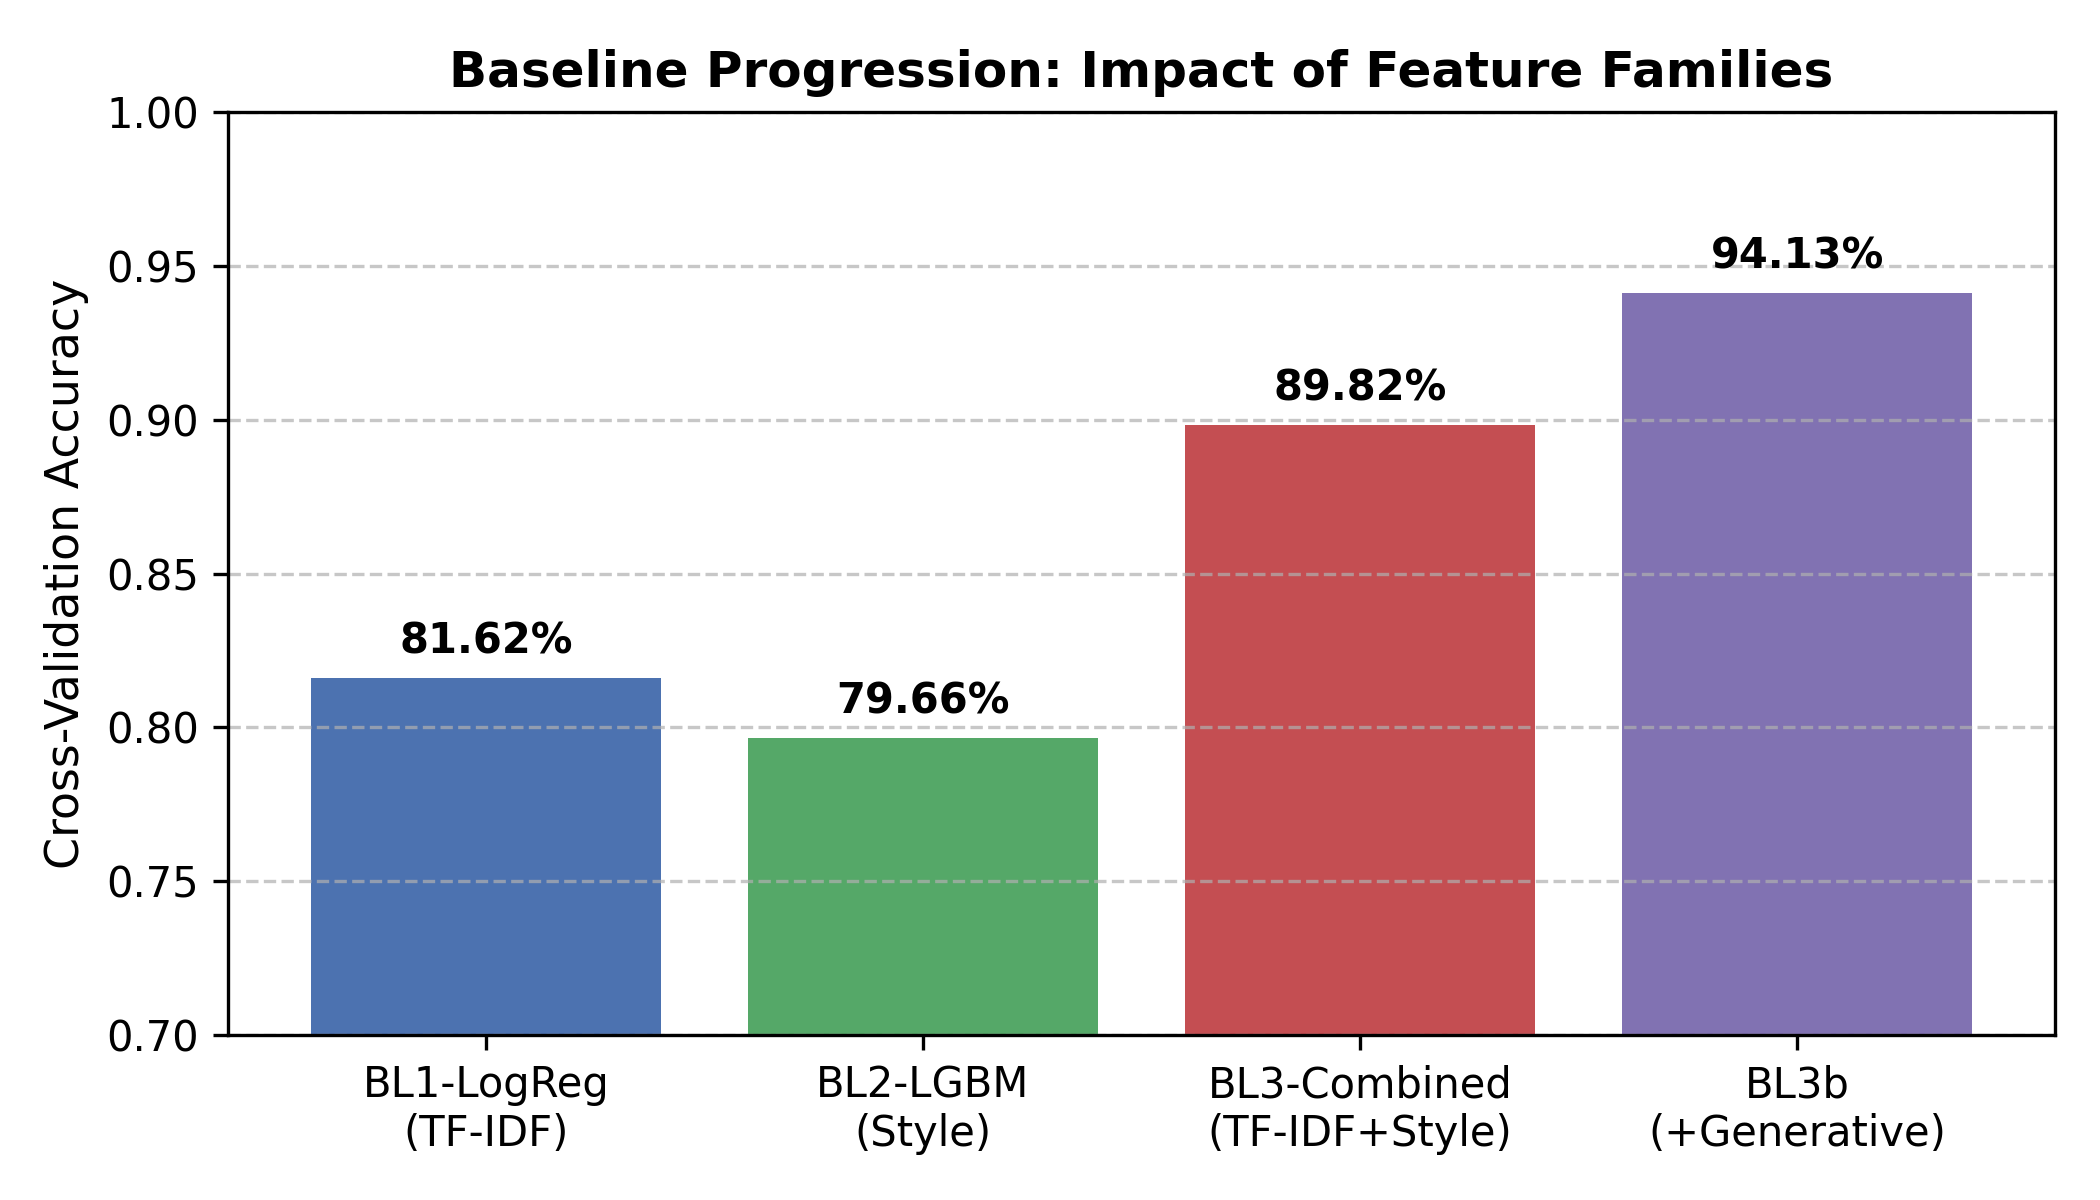
\includegraphics[width=0.65\textwidth]{baseline_progression.png}
\caption{Baseline progression showing the impact of successive feature families.}
\label{fig:baseline}
\end{figure}
\subsection{Champion Model and Noise-Floor Methodology}

Adding the Heaps' Law feature to BL3b yields the \textbf{Champion} (150,027 features). Multi-seed CV (seeds 42, 100, 2026, 777, 12345) established a noise floor of $94.15\% \pm 0.12\%$, giving a 2$\sigma$ acceptance threshold of \textbf{94.38\%}. \textbf{Kaggle: 96.00\%} (confirmed across three independent submissions).

\subsection{Systematic Feature Testing}

Six candidate feature families were tested against the Champion with leak-free CV. None cleared the 94.38\% noise floor:

\begin{table}[h!]
\centering
\caption{Post-noise-floor feature experiments (Champion baseline CV: 94.15\%).}
\label{tab:rejected}
\small
\begin{tabular}{@{}lccc@{}}
\toprule
\textbf{Feature Added} & \textbf{CV Acc} & \textbf{$\Delta$ vs.\ Base} & \textbf{Pass?} \\
\midrule
4th-order Quadgram & 94.20\% & +0.05 & No \\
Token Shape Stats & 94.12\% & $-$0.03 & No \\
Sliding Entropy & 94.17\% & +0.02 & No \\
Burstiness & 94.21\% & +0.06 & No \\
Graph Topology & 94.26\% & +0.11 & No \\
TF-IDF 200k & $\sim$94.22\% & +0.07 & No \\
\bottomrule
\end{tabular}
\end{table}

This confirms that the Champion's 150,027 features \textit{saturate} the discriminative signal available through token-level analysis.

\subsection{Dimensionality Reduction}

Compressing 150k TF-IDF features to 300 via TruncatedSVD reduced CV accuracy from 94.62\% to 94.41\%. Sparse exact n-gram matches encode highly specific lexical fingerprints that are blurred by dimensionality reduction. LightGBM already handles sparse matrices efficiently by not splitting on zero-valued features.

\subsection{Pseudo-Labeling}

Two independent attempts at self-training with high-confidence test predictions:

\begin{table}[h!]
\centering
\caption{Pseudo-labeling experiments (Champion Kaggle baseline: 96.00\%).}
\label{tab:pseudo}
\small
\begin{tabular}{@{}lcccc@{}}
\toprule
\textbf{Attempt} & \textbf{Threshold} & \textbf{CV Acc} & \textbf{Kaggle} & \textbf{Decision} \\
\midrule
Attempt 1 & 0.95 / 0.05 & 94.92\%$^*$ & 94.86\% & Rejected \\
Attempt 2 & 0.98 / 0.02 & 94.58\% & 95.53\% & Rejected \\
\bottomrule
\end{tabular}
\begin{flushleft}
\scriptsize $^*$CV estimate includes TF-IDF leakage (inflated by ${\sim}$0.4~pp).
\end{flushleft}
\end{table}

Both attempts inflated CV while \textit{degrading} Kaggle performance. The mechanism: self-training reinforces the model's existing confident predictions on easy examples without improving classification of ambiguous edge-cases. Pseudo-labeling was retired.

\subsection{Kaggle Leaderboard Summary}

\begin{table}[h!]
\centering
\caption{All Kaggle submissions.}
\label{tab:kaggle}
\small
\begin{tabular}{@{}lcc@{}}
\toprule
\textbf{Configuration} & \textbf{CV Acc} & \textbf{Kaggle} \\
\midrule
Champion LightGBM (150,027 feat.) & 94.15\% & \textbf{96.00\%} \\
Phase B Stacking (threshold 0.45) & 94.22\% & \textbf{96.00\%} \\
Phase 4 Pseudo-Labeling & 94.58\% & 95.53\% \\
Ultimate Model (all + pseudo) & 95.00\%$^*$ & 94.86\% \\
\bottomrule
\end{tabular}
\end{table}

\begin{figure}[h!]
\centering
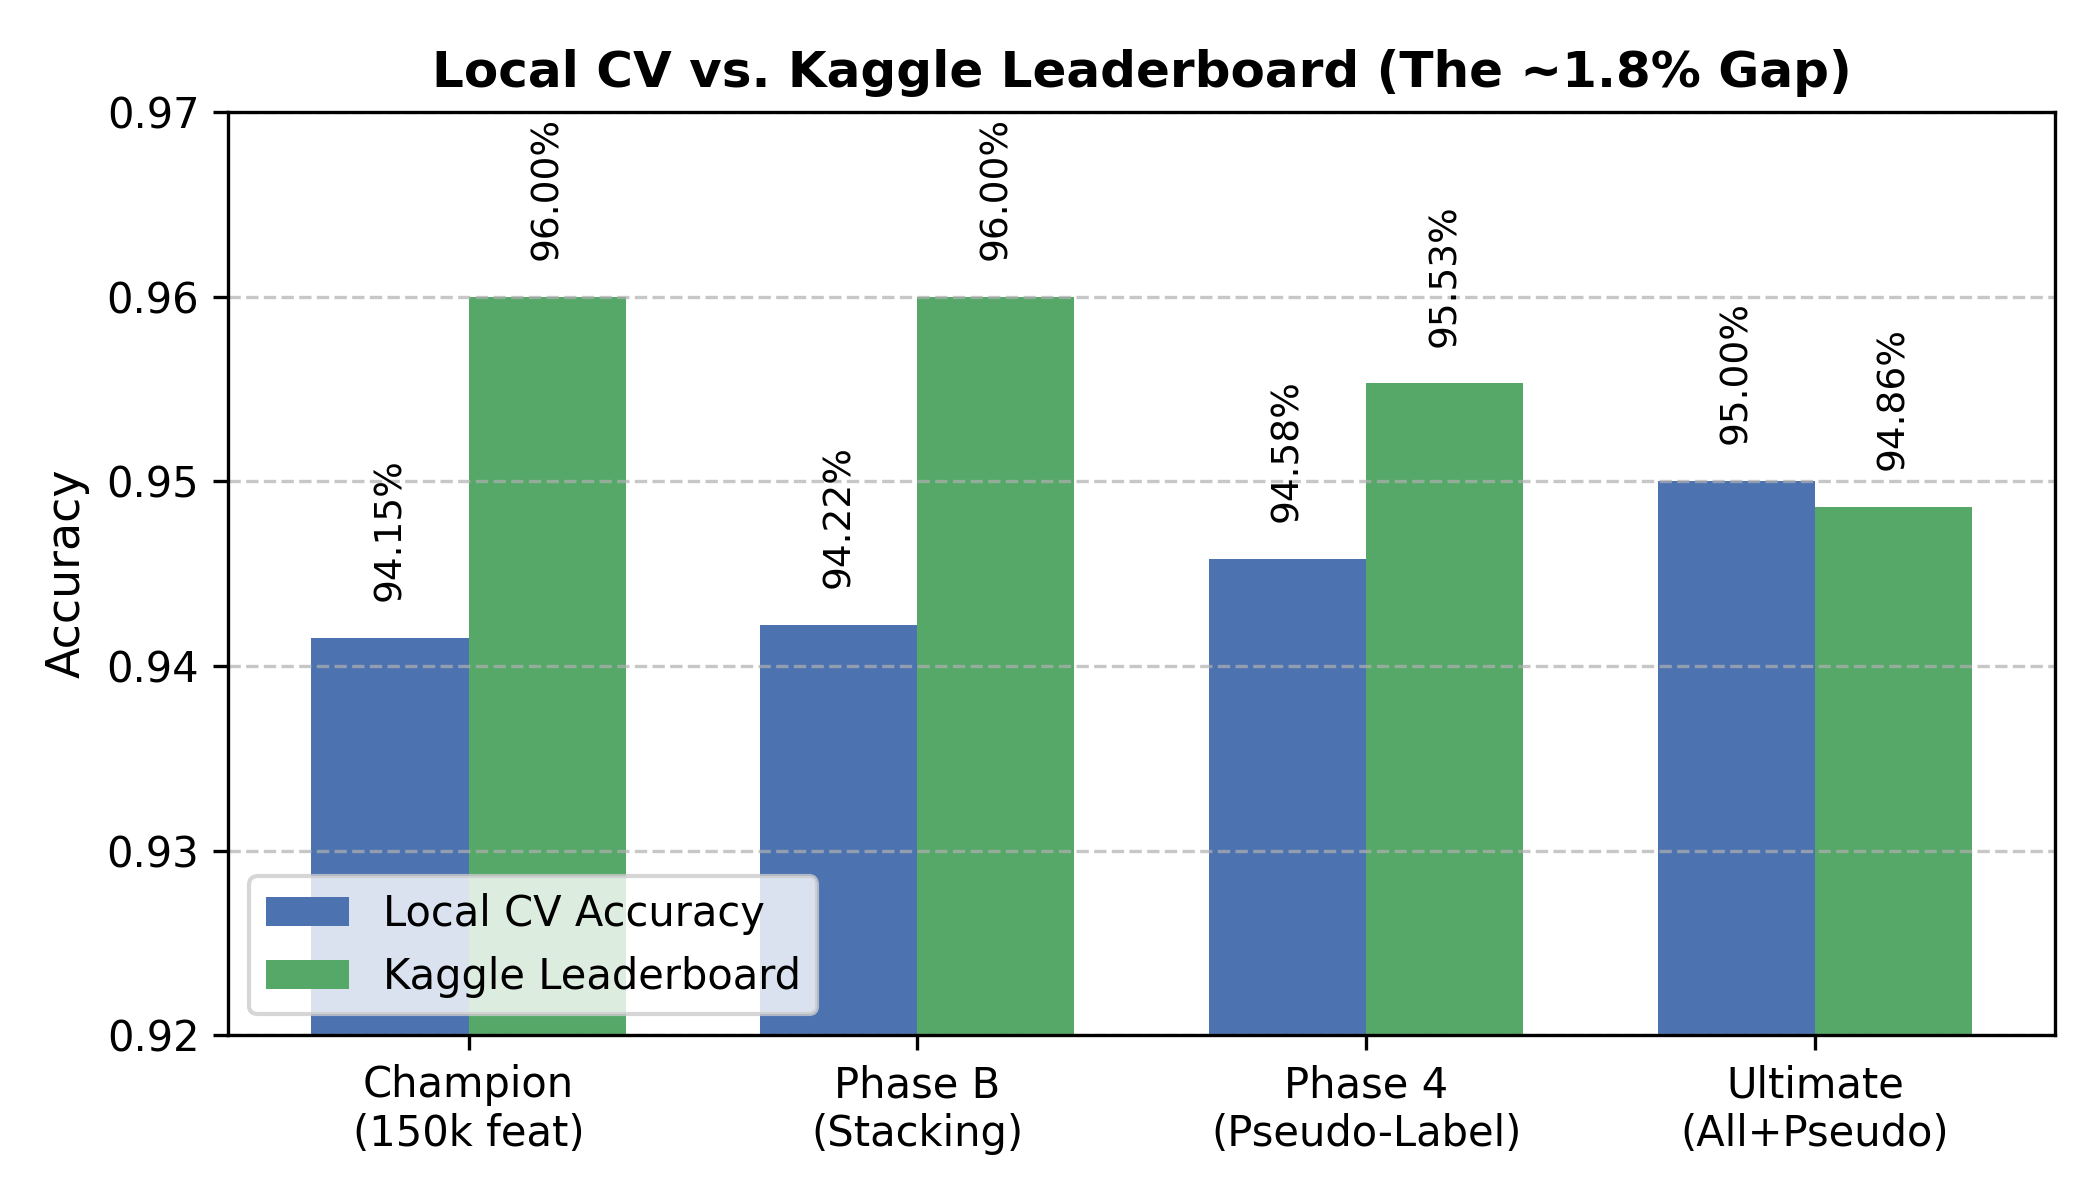
\includegraphics[width=0.65\textwidth]{cv_vs_lb.png}
\caption{Local CV vs. Kaggle Leaderboard performance for key configurations.}
\label{fig:cv_vs_lb}
\end{figure}

% ===================================================================
\section{Bonus Mark: Controlled Comparison}
% ===================================================================

We provide a strict controlled comparison demonstrating the impact of dictionary-based generative Markov features (Section~\ref{sec:gen}).

\textbf{Control} (BL3-Combined): TF-IDF (150k) + 6 base StyleFeatures $\to$ LightGBM.\\
\textbf{CV Accuracy: 89.82\%.}

\textbf{Treatment} (BL3b-Generative): TF-IDF (150k) + 18 ExtendedStyleFeatures + 8 GenerativeStyleFeatures $\to$ LightGBM.\\
\textbf{CV Accuracy: 94.13\% (+4.31~pp).}

Both use identical validation protocol (5-fold Stratified K-Fold, seed~42), identical LightGBM hyperparameters, and identical TF-IDF configuration. The \textit{only} difference is the addition of the generative and extended features.

\textbf{Justification}: TF-IDF captures token \textit{frequencies} but discards sequential dependencies. The Markov chain features recover this by computing class-conditional transition probabilities---directly measuring whether a document's token-to-token transitions look more like human writing or LLM sampling. The dictionary-based implementation avoids the infeasible $V^2$/$V^3$ dense matrices, and the LOO correction prevents training-set self-memorization.

% ===================================================================
\section{Discussion and Limitations}
% ===================================================================

\textbf{Why generative features dominate}: TF-IDF captures \textit{what} tokens appear; generative features capture \textit{how} they are sequenced. The log-likelihood difference (\texttt{ll\_diff}) directly quantifies which generative model better explains a document's transitions.

\textbf{Feature saturation}: Systematic testing confirmed the Champion feature set exhaustively captures the discriminative signal. All six candidate extensions were correctly filtered by the noise-floor methodology.

\textbf{CV/LB gap}: A consistent ${\sim}$1.8~pp gap between leak-free CV (${\sim}$94.15\%) and Kaggle (96.00\%) was observed, possibly reflecting distributional differences between training and test sets.

\textbf{Limitations}: (1)~Results are specific to this dataset's tokenization and may not generalize to raw text or unseen LLMs. (2)~No systematic hyperparameter optimization was performed. (3)~Post-noise-floor tests used a single CV seed. (4)~The 150k-dimensional sparse space carries overfitting risk, mitigated by LightGBM's regularization.

% ===================================================================
\section{Conclusion}
% ===================================================================

We developed a 150,027-feature classification pipeline achieving \textbf{96.00\% accuracy} on the Kaggle leaderboard. The most impactful contribution was memory-efficient, class-conditional Markov chain log-likelihood features (+4.31~pp over TF-IDF + stylometrics). A noise-floor methodology based on multi-seed CV prevented submission of statistically insignificant improvements. Two pseudo-labeling experiments provided clear evidence that self-training inflates CV without improving generalization. The combination of lexical, statistical, sequential, and information-theoretic signals saturates the discriminative capacity of token-level analysis for this dataset.

\end{document}
